\textbf{Problem 2:}

\singlespacing

Both the bus and you get to the bus stop at random times between 12 pm
and 1 pm. When the bus arrives, it waits for 3 minutes before leaving.
When you arrive, you wait for 15 minutes before leaving if the bus
doesn't come. What is the probability that you catch the bus?

\singlespacing
\singlespacing

In this problem we have that both the bus and you get to the bus stop
at a distributed random time between 12 pm and 1 pm. Let's define $X$
as the time that you get to the bus stop and $Y$ as the time that the
bus get to the bus stop. We have that $X$ and $Y$ are independent.

\singlespacing
\singlespacing

Imagine that we have a grid with height $60$ minutes and width $60$
minutes, and we have a point $(x, y)$ in the grid where $x$ is the
time that you get to the bus stop and $y$ is the time that the bus
get to the bus stop. We have that $x$ and $y$ are uniformly distributed
between $0$ and $60$.

\singlespacing
\singlespacing

So to solve this problem we only need to find the area of the grid where
the points $(x, y)$ satisfy the condition that you catch the bus.

\singlespacing
\singlespacing

These points are the points where $x-3 \leq y \leq x$ or $x \leq y \leq x+15$.
Because we have two scenarios:

\singlespacing
\singlespacing
\singlespacing

\textbf{Scenario 1:} The bus arrives first at time $y$ and you arrive
at time $x$, then you only get the bus if the bus arrives in the
last 3 minutes before you arrive, because the bus waits only for 3 minutes.

\singlespacing
\singlespacing
\singlespacing

\textbf{Scenario 2:} You arrive first at time $x$ and the bus arrives
at time $y$, then you only get the bus if the bus arrives before $x + 15$,
because you wait only for 15 minutes.

\singlespacing
\singlespacing

Then in the first scenario for each $x$ the valid $y$ are the $y$ between
$x - 3$ and $x$, and in the second scenario for each $x$ the valid $y$
are the $y$ between $x$ and $x + 15$. So ploting this three boundaries
$y = x - 3$, $y = x$ and $y = x + 15$ we have:

\singlespacing

\break

\begin{figure}[h]
    \centering
    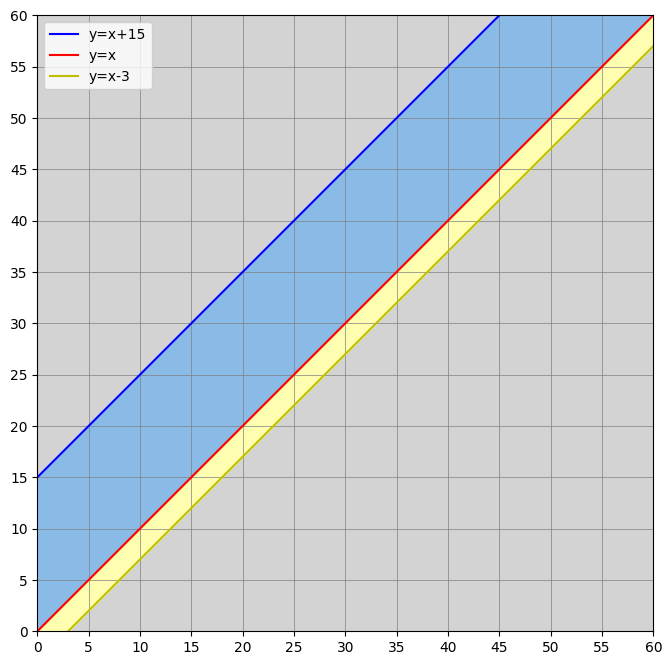
\includegraphics[width=0.4\textwidth]{img1.png}
    \caption{Plot of the three boundaries $y = x - 3$, $y = x$ and $y = x + 15$}
\end{figure}

\singlespacing
\singlespacing

So we have two areas, the yellow area and the blue area. The yellow area
represents the points in the first scenario and the blue area represents
the points in the second scenario. So the probability that you catch the
bus is the area of the yellow area plus the area of the blue area divided
by the area of the grid, because the points in the grid are uniformly and
independently distributed, so an specific area in the grid represent the
probability of that area to happen.

\singlespacing
\singlespacing

To calculate the yellow and blue areas we can subtract from the total
area of the grid the area of the triangle that is formed by the three
points $(3, 0)$, $(60, 0)$, $(60, 57)$ and the area of the triangle
that is formed by the three points $(0, 15)$, $(0, 60)$, $(45, 60)$.

\singlespacing
\singlespacing

\begin{figure}[h]
    \centering
    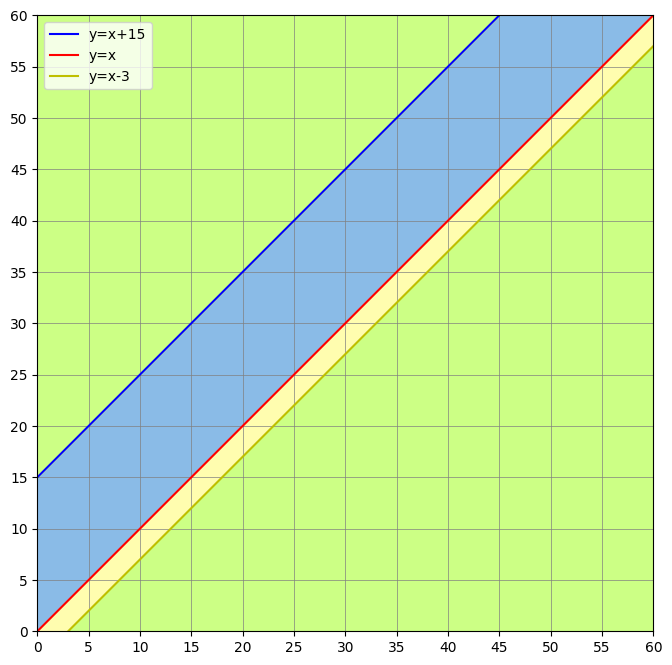
\includegraphics[width=0.4\textwidth]{img2.png}
    \caption{Plot of the two triangles in green}
\end{figure}

\break

Because the triangles are right triangles, we can calculate the area
of the triangles as the half of the product of the height and
its base, the first
triangle has a base and height of $60 - 3 = 57$,
so the area of the first triangle is $\frac{57 \cdot 57}{2} = 1624.5$,
and the second triangle has a base and height of $60 - 15 = 45$,
so the area of the second triangle is $\frac{45 \cdot 45}{2} = 1012.5$.

\singlespacing
\singlespacing

Because the total area of the grid is $60 \cdot 60 = 3600$, then the
yellow plus blue area is $3600 - 1624.5 - 1012.5 = 963$.

\singlespacing
\singlespacing
\singlespacing

So the probability that you catch the bus is $\frac{963}{3600} = 0.2675$.